\section{Internship organization} 
	\subsection{Introduction}

This section is meant to be added to the University version of this documentation. It will be written as Erwan Ulrich and will focus on the different aspects of the organization of the project. The following text will also be written with a more personal and more critical point of view as a mean of self analyze.

	\subsection{The BFH and The GNU Taler package}
My internship was supervised by both the Berner Fachhochschule (Bern University of Applied Sciences) and Christian Grothoff who is the maintainer for multiple GNU packages among which the GNU Taler package.

Founded in 1997,  is a non-profit public higher education institution located in the large town of Bern (population range of 50,000-249,999 inhabitants). Berner Fachhochschule (BFH) is a medium-sized (uniRank enrollment range: 6,000-6,999 students) coeducational higher education institution. Berner Fachhochschule (BFH) offers courses and programs leading to officially recognized higher education degrees such as bachelor degrees in several areas of study.

GNU is a politically engaged, free software and mass-colaboration project that was created by Richard Stallman in 1983 at the MIT. It aims to produce and distribute free softwares to help citizens keep control over their computers and digital activities. Most softwares produced by the GNU project share the same GNU General Public License that give rights for it to be run, shared, studied and modified. This subscribes to the global philosophy and political engagements of the GNU project.

Christian Grothoff is professor at the BFH as well as the main developer and team leader of the GNU Taler package.
The Taler project is an electronic payment system under development at Inria.
It provides accountability to ensure business operate legally, while also respecting civil liberties of citizens. Taler is based on open standards and free software.
Taler was built with the goal of fighting corruption and supporting taxation. With Taler, the receiver of any form of payment is easily identified, and the merchant can be compelled to provide the contract that was accepted by the customer. Governments can use this data to tax businesses and individuals based on their income, making tax evasion and black markets less viable. 

I was positioned under the supervision of Mr Grothoff with the task of conceiving, coding and deploying a tool that would help secure database exchanges as a part of the Taler payment system development.  
	\subsection{Calendars}
	
The	SchemaFuzz project has had since its genesis a quiet clear view of how the development should evolve. The desired features have been discussed and the big picture had been designed to fit the time that the main developer had for his work at this position.
The project had to pass trough different phases of development that are detailed in the following time line diagram. 

		\bigskip
		\begin{figure} [h!]
			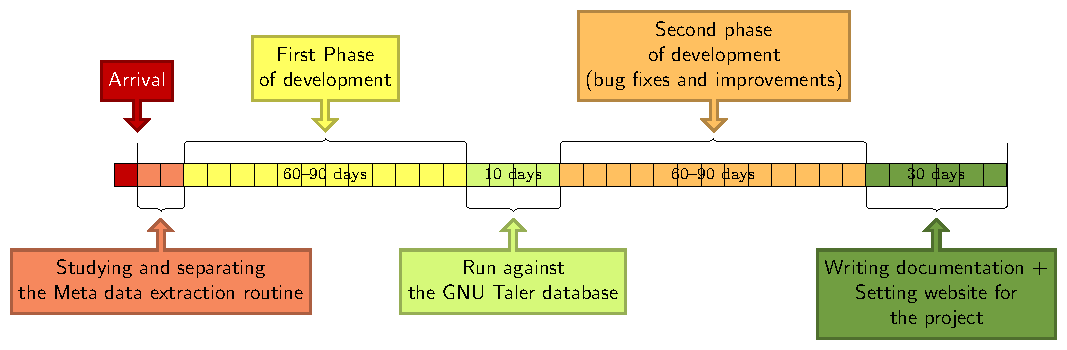
\includegraphics[width=\textwidth]{timelineDiagram.pdf}
			\caption{Originally planned organization}
		\end{figure}
		\bigskip


Some of the tasks of the above time line were completed on time, some others were delivered late, and some were delayed in the time line because of the previous point.
In the end, the project was lead in a way that is best described by the following time line diagram.

		\bigskip
		\begin{figure} [h!]
			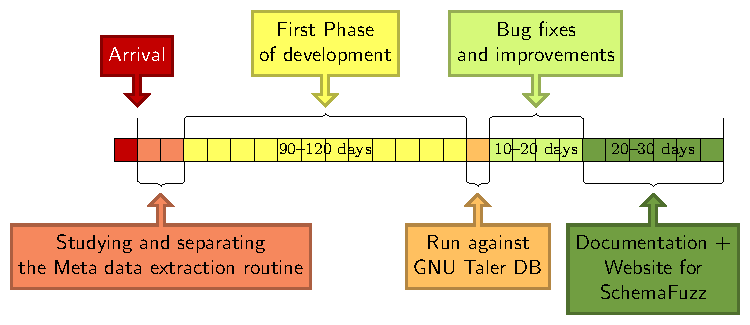
\includegraphics[width=\textwidth]{timelineDiagram2.pdf}
			\caption{Organization results}
		\end{figure}
		\bigskip

Those two diagrams differ on some points.There are several reasons that explain why this project could have been lead in a better way. They will be detailed and discussed in the next section. 

	\subsection{General Organization}
The following organizational points help explain why the SchemaFuzz project did not meet all of its defined goals.
It is also a personal reminder of what should be improved in my work habits and general organization when leading a project of such a large size. 
	
	\begin{itemize}
	\item{Defining tasks/features as daily/weekly sub goals}
	\item{Improving general project planning}
		\begin{itemize}
		\item{Include the test writing in the planning as a "real" task}
		\item{Build the project's code structure beforehand}
		\item{Decide what approach to use for each component beforehand}
		\item{Decide for each component what technologies should be used beforehand}
		\end{itemize}
	\item{Setting up more fluid communication}
	\end{itemize}		

	\subsection{Positive outcomes}
Throughout the development of the project, I have had the chance to acquire many new capacities and improve many of my own skills. I will give more insights on what this project and, more generically, what this internship as a developer for a GNU package, has brought me.
Apart from the Java language, which I was already familiar with, I also had the chance to get my hands of new technologies (or technologies I never really had the chance to practice in real conditions). 

		\subsubsection{Technical aspect}
		
		\paragraph{Java language}
In many ways, this project has been a real challenge. But the main difficulty that I encountered was the technical challenge that rose up when the project started. Indeed, it was my first time conducting a project of the size of SchemaFuzz. The size of the project and the fact that I was the only one developing the tool implied that every aspect of the project, independently of the language that was used for each module, had to be imagined and implemented with my two hands.
Even if I was already accustomed to Java programming, I got struck by the complexity and the architecture of a "real" in-production software like SchemaSpy which I had to look into to get the meta data extraction routine.
This was my first improvement. Code structure. Even if my coding capacities can still be perfected in many ways, I feel like understanding/re-using complex and well structured code gave me a much better idea of what "good code" really is. Integrating these concepts empowered my development skills and I am now much more confident about it.

			\paragraph{SQL language}
SchemaFuzz is a database fuzzer. Naturally, A major component of the work for its development was to create and handle SQL requests and responses. In order to do that, I had to document myself for a while as I was lacking some knowledge on databases in general. After gaining a better understanding of how databases operate theoretically, I had to go into more depth concerning the inner structure of constraints and the way data types are encoded for most DMBS.
This brings me to my next point regarding the handling of SQL in this project.

			\paragraph{DBMS(PostgreSQL)} 
SchemaFuzz's first and foremost import goal is to help in the debugging and maintenance of the GNU Taler payment system. GNU Taler databases are managed by the PostgreSQL DBMS. Therefore, the natural choice of technology for SQL management in this project was obvious.
Not having ever worked with PostgreSQL before, I had to adapt my habits when dealing with the DBMS itself.
By doing so, and stumbling on error messages I had never seen before, I had the chance to get into more depth in the structure of DBMSes in general. In particular, I had to get my hands on the inner PostgreSQL tables in order to understand how different databases were managed within the same environmental.

			\paragraph{Shell/Bash Scripting} 
As a part of the development of the analyzer for SchemaFuzz, I have had the chance to build up several bash scripts. This  was to me a true pleasure as well as very instructive.
Spending some time on writing parsing script had me look into how parsing is usually implemented for such jobs.
Having this experience with me, I now better understand how each and every component of a same project connects to each other. 
Even though I was aware of the power of scripting in general, I have now come to understand how much of a crucial skill it is to understand and be able to write scripts when working in a Linux environment.
In the big picture, I feel like I have earned a precious asset by practicing scripting on a technical level. This also gave me the chance to develop my own script in the frame of personal use in my own environmental. Going through more conceptual and theoretical documents on what scripting really is and how it should be used.
   			
			 \paragraph{LateX}
By writing this documentation, I had to learn how to create and process properly presented and properly styled scientific documents. In this process, I have first learned and then practiced LateX as well as the very handy Tikz and metaUML packages used for graphical representations.
Creating and implementing (in this case) graphics I did not consider to be a real coding challenge, but some of them proved me terribly wrong. Spending time on finding the right syntax for what I wanted to show strengthened my project management skills and comforted me in the belief that presentation and creation of a project are two sides if the same coin and that both should be treated with the same amount of seriousness.  			  
	

		\subsubsection{Human aspect}
		
			\paragraph{Languages}
The development of my project was conducted in German-speaking environment, which is a language I am not very familiar with. 
This lead to having any kind of communication both regarding the project and other subjects in English. This participated in my improvement in both oral and written English (this document is also an excellent training for written content) as well as my overall comprehension.
Apart from the pure linguistic point of view, discussing complex topics in English gave me the keys to expressing ideas and concept in a more concise and clearer way. 			

			\paragraph{Political maturity}
Disclaimer. With this paragraph, I am not pushing forward any idea in particular, all I intend to do is explain with more detail and insights on how rich the environment was during this internship.			
			
Surprisingly, I have had the chance to meet many people that shared various political points of view regarding computer science and technologies. In these subjects it was a truly enriching process to debate things such as morality, ethic or freedom.
Some other topics that are further away from science were brought up such as vegan-ism, green energies, or anarchism.
I hold very dearly the moments I shared speaking and confronting my own ideas because I feel like this has allowed me to gain maturity in my political positions.		
	
	\clearpage

	\subsection{Conclusion}
   
The development of SchemaFuzz and my work for GNU Taler was spread out on a 6 months duration.
Within this time lapse, I have discovered the fields of research and real software development.
This discovery has been very beneficial to me in the sens that it gave me the chance to acquire experience both on the theoretical and technical sides as well as mastering some new technologies and new aspects in the field of computer science in general.

My work for GNU Taler was primarily to imagine,conceptualize and develop a database oriented fuzzing tool. 
First, I focused on bringing the software from a shape of "general idea" that was given to me by my internship supervisor to a concrete and structured project. In the process of creation, I started with defining what precise features were critical and with what technology they would be implemented.

The main task of SchemaFuzz is to inject malformed data into a specific database in order to trigger crashes or unexpected behavior from the program that uses the content of this database.
By working on this project for the past 6 months, I have brought it to a point where it fulfills its main task. I have uses a sample database contain content with a wide variety in terms of data types to test the project all along the course of the development. However, the application is meant to evolve to a more advanced state. Such a big project requires much more time than what I had to be fully operational.

Finally, I am convinced that the realization of this project was a truly rewarding experience on all academical, technical and human aspects. All the knowledge acquired as GNU developer strengthened the concepts I had learned in my academical courses. Moreover, this internship is an excellent social experience thanks to the amount of contact with very bright professors, PhD students and other interns.     
   
\clearpage

\section{Acknowledgments}

I would like to express my deepest appreciation to those you helped throughout the progress of my internship and development of my work.
A special gratitude I give to my project supervisor Mr Christian Grothoff for his technical and moral support during my work as well as for his infinite patience.
Furthermore, I would like to acknowledge with much appreciation the staff at BFH for their warm welcome and more specifically Ms Jost for her help regarding administrative duties.
A special thanks goes to Julius Bunger for his moral support and for sharing his experience with me on many subjects and levels.
I also have to appreciate the opportunity of working in a calm space that was given to me by the Dezentrale.
I would also like to thank all my friends for their wise counsel and more specifically Leo Barouh, Jeremy Wuille and Ruben de Barros for their unfailing presence in delicate situations.   
Finally, I can not express enough gratitude to my dad that gave me all his support when it was needed the most as well as for his help regarding the coordination of my project especially in the writing of this report.        